\section{Homophily: \emph{"Birds of a feather flock together"}}
\label{sec:homophily}
%\vspace{-0.2cm}
%\begin{center} \emph{Birds of a feather flock together} \end{center}
%\vspace{0.1cm}

Homophily refers to the tendency of individuals to connect to similar others: two individuals (and thus their corresponding nodes in a social network) are more likely to be connected if they share common characteristics~\cite{mcpherson2001birds,lazarsfeld1954friendship}. The characteristics often considered are inherent to the individuals: they may represent their social status, their preferences, their interest, ... A related notion is the one of {\it assortativity}, which is slightly more general as it applies to any network, and not just social networks, and refers to the tendency of nodes in networks to be connected to others that are similar in some way.

A definition of homophily has been proposed in~\cite{la2010randomization}. However, this definition, which relies on a single characteristic (as age or gender), does not allow one to assess whether latent models for link prediction capture the homophily effect or not. We thus introduce a new definition of homophily below, which directly aims at this:
%
\begin{definition}[Natural Homophily]
	Let $\mathcal{M}=\{\mat{F},\mat{\Phi}\}$ be a link prediction model as defined above and $s$ a similarity measure between nodes. We say that \emph{$\mathcal{M}$ captures the natural homophily effect} iff, $\forall (i,j,i',j') \in V^4$:
%
\begin{equation}
s(i,j) > s(i',j')  \implies \pr(y_{ij}=1 \mid \mathcal{M}) > \pr(y_{i'j'}=1  \mid \mathcal{M}) \nonumber
\end{equation}
%
A model which verifies this condition is said to be \emph{naturally homophilic}.
\end{definition}
%
As one can note, this definition directly captures the effect "if two nodes are more similar, then they are more likely to be connected The model $\mathcal{M}$ considered can either be regarded in a purely generative setting, or be learned from the data. The above definition encompasses both cases, the parameters $\mat{F}$ and $\mat{\Phi}$ being either generated or learned. Furthermore, in some cases, for example when one has access to users' interest or social information, one may use \textit{a priori} representations of nodes as well as given weight matrix between them. This situation corresponds to the case where the matrices $\mat{F}$ and $\mat{\Phi}$ are given, the variables $y_{ij}$ still being generated according to Eqs.~\ref{eq:link-ilfm} and \ref{eq:link-immsb}. The definition of homophily given above is still applicable in this setting.

The similarity function assesses to which extent two nodes share the same characteristics. The parameters $\mat{F}$ and $\mat{\Phi}$ respectively capture latent characteristics of nodes and weights (or correlations) between the dimensions of these representations; a natural similarity between node characteristics is thus provided by:
%
\begin{equation}
s(i,j) = \mat{f}_{i} \mat{\Phi} \mat{f}_j^\top
\label{eq:natural-sim}
\end{equation}
%
From this, one can state the following property:
%
\begin{proposition}[]
ILFM is naturally homophilic under the similarity measure defined by Eq.~\ref{eq:natural-sim}.
\end{proposition}
%
\noindent The proof of this proposition is straightforward, and directly stems from the fact that the sigmoid function is strictly increasing.

The situation for IMMSB is slightly different inasmuch as the selection of classes from the latent class representations may lead to reversing the order between two pairs of nodes for the similarity and the probability of connecting the nodes. Indeed, IMMSB is \textit{not} strongly homophilic. This said, IMMSB still captures an homophily effect in the following sense:
%
\begin{proposition}[]
Let $s$ be the similarity measure defined by Eq.~\ref{eq:natural-sim}. IMMSB is \emph{weakly homophilic}, \textit{i.e.}  $\forall (i,j,i',j') \in V^4$:
%
\begin{align}
&s(i,j) > s(i',j')  \implies \nonumber \\
%&\mathbb{E}_{\pr(z_{ij},z_{ji}|\mathcal{M})}[\pr(y_{ij}=1 \mid \mathcal{M})] > \mathbb{E}_{\pr(z_{ij},z_{ji}|\mathcal{M})}[\pr(y_{i'j'}=1  \mid \mathcal{M})] \nonumber
&\mathbb{E}_{\pr(z|\mathcal{M})}[\pr(y_{ij}=1 \mid \mathcal{M})] > \mathbb{E}_{\pr(z|\mathcal{M})}[\pr(y_{i'j'}=1  &\mid \mathcal{M})] \nonumber
\end{align}
\end{proposition}
%
\noindent \textbf{Proof} We have:
%
\begin{align}
&\mathbb{E}_{\pr(z_{ij},z_{ji}|\mathcal{M})}[\pr(y_{ij}=1 \mid \mathcal{M})]\nonumber \\
&= \sum_{k,k'} \phi_{k,k'} \pr(z_{ij}=k|\mathcal{M}) \pr(z_{ji}=k'|\mathcal{M}) \nonumber \\
&= \sum_{k,k'} \phi_{k,k'} f_{ik} f_{jk'} = \mat{f}_i \mat{\Phi} \mat{f}_j^\top \nonumber
\end{align}
%
where $f_{ik}$ denotes, as before, the element of $\mat{F}$ at the $i^{th}$ row and $k^{th}$ column and where the second equality stems from the definitions of $z_{ij}$ and $z_{ji}$. Hence $\mathbb{E}_{\pr(z_{ij},z_{ji}|\mathcal{M})}[\pr(y_{ij}=1 \mid \mathcal{M})]$ varies in the same way as $s$. \hfill$\Box$ \\

The above development shows that both ILFM and IMMSB can capture the homophily effect, with a strict adherence to it in the case of ILFM, and a looser one for IMMSB.


~\\
\textcolor{red}{Addtitional work (need to change to strongly homophily into natural homophily, and avoid talking about estimating parameters, no need here bacause no observation on real features of the data). Also I propose (but eventually, I think its a detail) to remove the concept to strong/weak property for now because, we actually identity a link prediction model by $\{\phi, F\}$ so $Z$ variable are dummy and implicitely marginalized.}
~\\


The homophily previously defined is somehow trivial in the sense that in latent models we saw that the likelihood to generate a link $\p(y_{ij} |\Theta)$ is the parameter of the bernoulli kernel in binary relationship. Hence, if we choose the similarity for the homophily effect as this exact likelihood the order is tribially preserved. A more interesting question is to look if the models are homophilic when the similarity is based only on the latent features. In other words the question is to compare the gramm matrix defined on latent feaures and the bilinear form induce by the weight matrix $\Phi$ that brings the latent feature space into the probability space of the links likelihood. We defined the latent similariry between nodes as the inner product of their latent features:
\begin{equation}
s(i,j) = \mat{f}_{i} \mat{f}_j^\top
\label{eq:latent-sim}
\end{equation}

We now define the latent homophy as follow:

\begin{definition}[Latent Homophily]
	Let $\mathcal{M}=\{\mat{F},\mat{\Phi}\}$ be a link prediction model as defined above and $s$ a similarity  measure between nodes and which only depend on $\mat{F}$. We say that \emph{$\mathcal{M}$ captures the latent homophily effect} iff, $\forall (i,j,i',j') \in V^4$:
%
\begin{align}
&s(i,j) > s(i',j')  \implies \nonumber\\
&\E_\Phi[\pr(y_{ij}=1 \mid \mathcal{M})] > \E_\Phi[\pr(y_{i'j'}=1 \mid \mathcal{M}) \nonumber
\end{align}
%
A model which verifies this condition is said to have \emph{latent homophily}.
\end{definition}
%

In the rest this section we will consider that reference the similarity measure $s$ refers to equation \eqref{eq:latent-sim}, the latent similarity.

\begin{proposition}[]
	ILFM is and iMMSB does not satisfy the latent homophily under the latent similarity.
\end{proposition}

\noindent \textbf{Proof} We have thath $\Phi$ are i.i.d either from beta or normal distribution. Thus we have that $\E[\Phi] = \mu \unit$, where $\unit$ is matrix with one everywhere and $\mu$ a constant corresponding to the mean of the prior over weight. Then we have:
%
\begin{align}
&\mathbb{E}_{\Phi}[\pr(y_{ij}=1 \mid \mathcal{M})] \nonumber \\
&= f_i \E[\Phi]f_j = \mu f_i \otimes f_j  \nonumber \\
&= \mu (\sum_k f_{ik}f_{jk} + \sum_{k\neq k'} f_{ik}f_{jk'} ) \nonumber
\end{align}
%
Where $\otimes$ is the outer product. Whitin the last equation, it is easy to find a counter example where the similarity order is lost by the outer product. Example fall in the stochastic block model case (which is a special case of both model),  when two nodes have a disjoint feature vectors against one that have only one membership in common. \hfill $\Box$ \\

This proposition means that the latent features generated or learn for both model will not encode the classical vision of homophily, which says that if two individuals have similar feature, they will be likely to connect. This proposition also hilghight the fact the latent feature of iMMSB and ILFM can't be interpreted out of the box as communities where links occur more likely when two individuals has identical membership.

In the contrary, one can imagine that if $\Phi$ is constrained such that latent homophily is true, one can directly interpret the latent features as communities indicator. This is basically what is done is this paper \cite{AMMSB} to find overlapping communities within the MMSB models. The authors renamed the constraint MMSB to a-MMSB, standing for assortative MMSB. \textcolor{red}{I have the proof with the matrix normal as an example, but a-MMSB is even simpler --- $\phi_{kk'}=0$ if $k\neq k'$.}

In figure \ref{fig:gen_blocks}, we show a clustering result form MMSB based on the blockmodels. We choose the a cluster of assignment for each node which represent the latent feature with highest probability. Thus it appears that MMSB capture the structural equivalence of the underlying networks.

\begin{figure}[h]
	\centering
	
	\minipage{0.17\textwidth}
	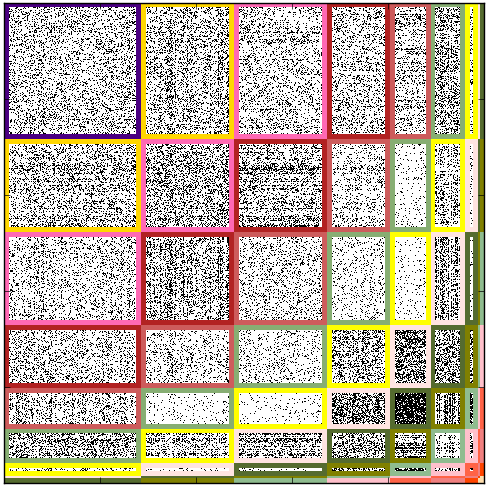
\includegraphics[width=2.94cm, height=3cm]{img/M_g_peaks/figure_6}
	\endminipage
		\minipage{0.17\textwidth}
	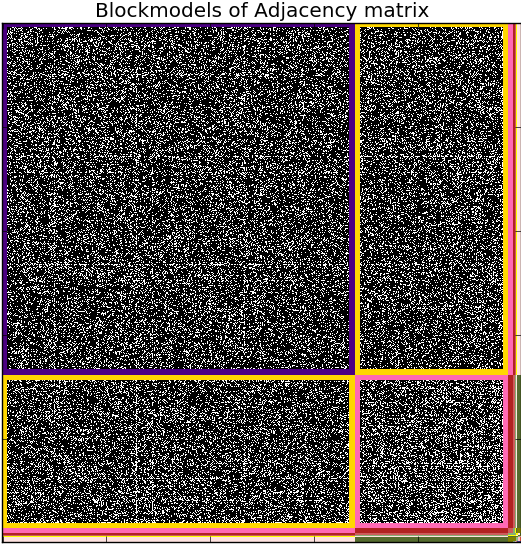
\includegraphics[width=2.94cm, height=3cm]{img/M_g_power_law/figure_6}
	\endminipage
	\minipage{0.17\textwidth}
	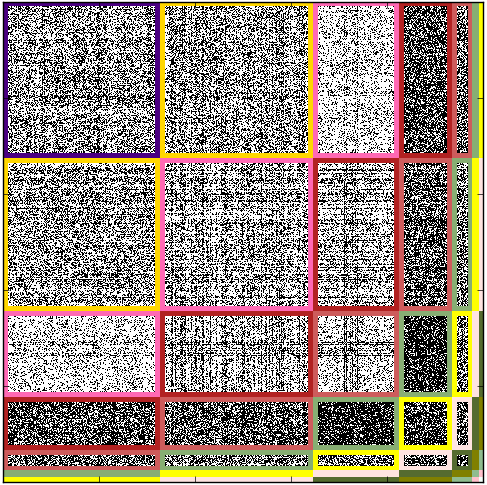
\includegraphics[width=2.94cm, height=3cm]{img/M_g_regular/figure_6}
	\endminipage
	%\vspace{-0.3cm}
    \vspace{0.3cm}
	\minipage{0.16\textwidth}
	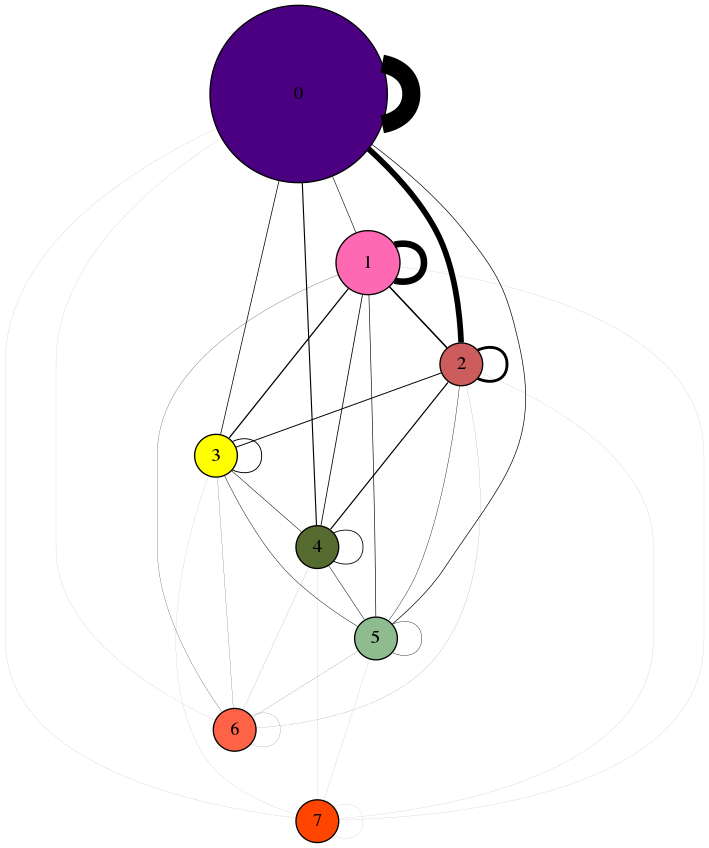
\includegraphics[width=3.5cm, height=4cm]{img/M_g_peaks/graph_dot}
	\endminipage
		\minipage{0.16\textwidth}
	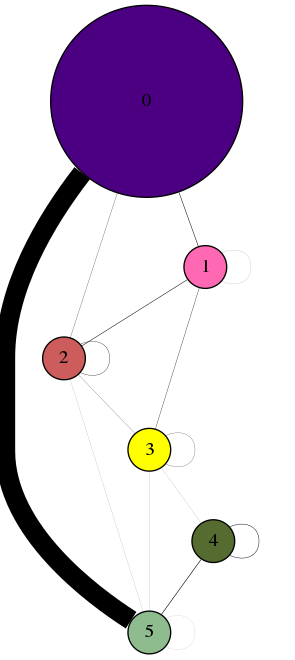
\includegraphics[width=3.5cm, height=4cm]{img/M_g_power_law/graph_dot} 
	\endminipage
	\minipage{0.16\textwidth}
	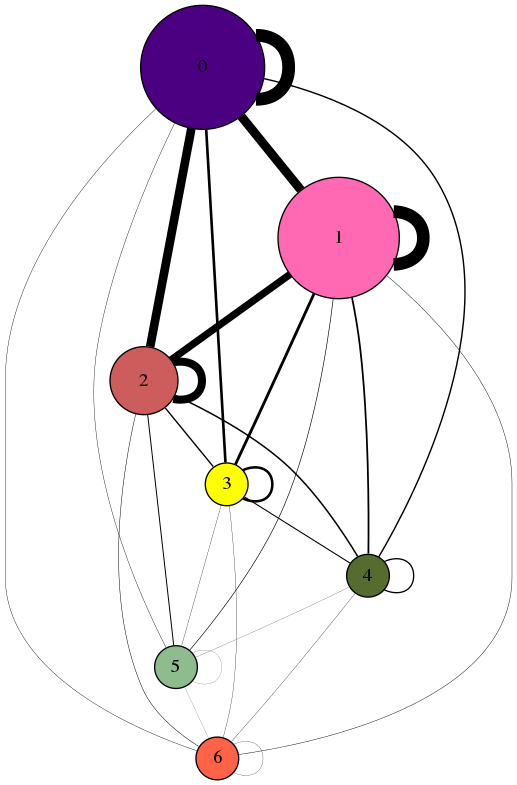
\includegraphics[width=3.5cm, height=4cm]{img/M_g_regular/graph_dot}
	\endminipage
	\caption{}
	\label{fig:gen_blocks}
\end{figure}


 We now turn to the burstiness effect.
